%
% problemstellung.tex -- Beispiel-File für die Beschreibung des Problems
%
% (c) 2020 Prof Dr Andreas Müller, Hochschule Rapperswil
%
\section{Problemstellung
\label{taylor:section:problemstellung}}
Um die numerische Approximation an einem konkreten Beispiel zeigen zu können wird hier die logistische Differentialgleichung analysiert.
Es handelt sich hierbei um eine begrenze Wachstumsfunktion. 
Mit dieser Differentialgleichung können zum Beispiel der Verlauf einer Krankheit, der Lebenszyklus eines Produktes oder auch Zerfallsprozesse beschrieben werden. Die Parameter der logistischen Differentialgleichung 
\begin{align*}
	y' &= k\cdot y(L-y) 
	&&\text{mit der Anfangsbedingung}
	&y(0) &= 0.5
	\label{taylor:section:logistifunction}
\end{align*}
haben die Bedeutung: $L$ = Endwert und $k$ = Wachstumsrate.
Wir normieren den Endwert $L$ auf 1.
Der Endwert entspricht zum Beispiel der Anzahl Infizierten am Ende einer Epidemie.
\index{Infizierte}%
\index{Epidemie}%
In der Abbildung ~\ref{taylor:section:fig:DGLDarstellung} ist zu erkennen, dass der Wachstumsfaktor $k$ bestimmt, wie steil die Funktion wird.
Es existiert nun also für jeden möglichen Punkt der logistischen Funktion in diesem Richtungsfeld ein genau definierter Wert $k$.
Um das $k$ zu bestimmen, müsste die Differentialgleichung gelöst werden.
Möchte man dies umgehen, weil das zum Beispiel viel Rechenaufwand bedeuten würde, bzw. für einen Computer viel Rechenzeit bedeutet, kann die Lösung der Differentialgleichung mit kleinen Schritten erarbeitet werden.
Dazu vergleichen wir die beiden Inkrementfunktionen Runge-Kutta- und Taylor-Approximation.
\index{Runge-Kutta-Verfahren}%
\index{Taylor-Approximation}%
Der Wachstumsfaktor
\index{Wachstumsrate}%
\begin{equation}
k=\frac{-\ln{(\frac{1}{y}-1)}}{x}
\qquad
\left(\text{aus der Lösung $y(x)=\displaystyle\frac1{1+e^{-kx}}$}\right)
\end{equation}
ist also sowohl von $x$ als auch von $y$ abhängig, allerdings nur durch $x$ und $y$ berechenbar wenn die Differentialgleichung gelöst wurde.
Die Taylor-Approximation darf sich dieser Formel deshalb nicht bedienen.

\begin{figure}
	\centering
	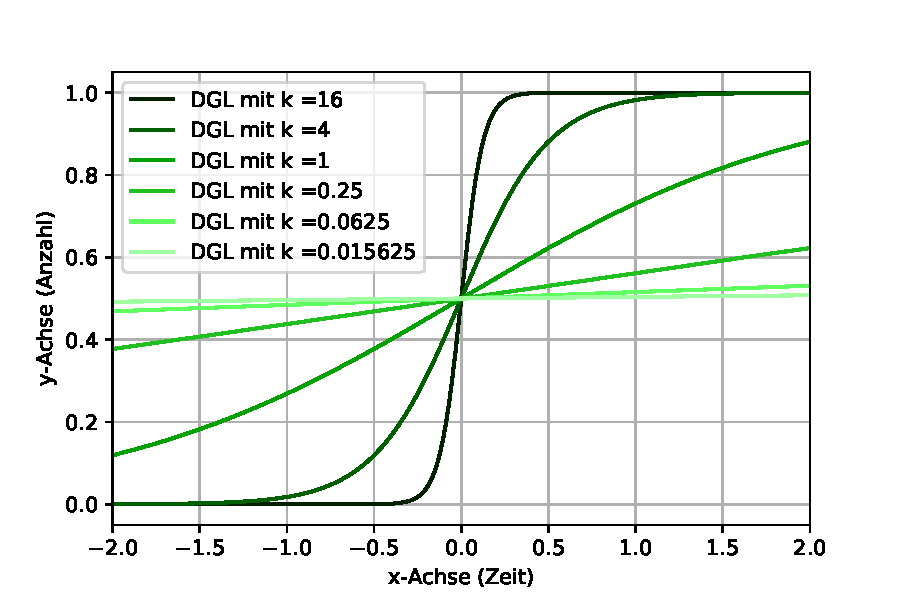
\includegraphics[width=12cm]{papers/taylor/taylorPictures/DGLDarstellung.pdf}
	\caption{Logistische Funktion in Abhängigkeit von k}
	\label{taylor:section:fig:DGLDarstellung}
\end{figure}

\section{Das Taylor-Verfahren}
\label{taylor:subsection:Vorgehen}
Wir benötigen für die Taylor-Approximation die Ableitungen bis zur $n$-ten Ordnung.
Also bis zur Ordnung, mit welcher wir die Differentialgleichung approximieren wollen.
Wie man auf diese kommt, ist in Kapitel \ref{grundlagen:hoehere-ableitungen} beschrieben.
Man erhält die Gleichungen

\begin{equation}
\begin{aligned}
y'&=k\cdot (y-y^{2})\\
y''&=k\cdot (y'-2y'\cdot y)\\
y'''&=k\cdot (y''-2y''\cdot y+y'^{2})\\
y''''&=k\cdot (y'''-2y'''\cdot y+3y''\cdot y')\\
y'''''&=k\cdot (y''''-2y'''\cdot y+4y''\cdot y'+3y''^{2})\\
\end{aligned}
\end{equation}
durch Ableiten der logistischen Funktion.

Die allgemeine Formel der Einschritttheorie sieht so aus:
\begin{equation}
y(x+h) = y(x) + h\cdot f(x,y),
\end{equation}
wobei die Funktion $f(x,y)$ der Approximationsfunktion entspricht, mit welcher der nächste Punkt berechnet wird.

Beim Taylor-Verfahren soll nun also mit kleinen Schritten der Verlauf der Funktion ausgehend von einem Anfangswert ermittelt werden.
Die Taylor-Reihe
\begin{equation}
f_{T}(x,a)
=
\sum_{n=0}^{\infty}{\frac{f^{(n)}(a)}{n!}}\cdot (x-a)^{n}
\label{taylor:section:taylor}
\end{equation}
%$f_{T}(x,a)$ = Taylor Funktion
setzt sich zusammen aus der korrekten Gewichtung der Ableitungen bis zur gewünschten Ordnung.
Je höher der Grad der Auswertung der Taylor-Reihe gewählt wird, desto grösser ist der Bereich um den Auswertungspunkt $a$ in welchem die Approximation mit der logistischen Funktion übereinstimmt.
Am Auswertungspunkt wird nun mit der beschriebenen Approximation der nächste Punkt berechnet.
Dieses Verfahren mit der Inkrementfunktion
\index{Inkrementfunktion}%
\index{Ableitung}%
\begin{equation}
y(x+h)
=
\sum_{n=0}^{g}{\frac{f^{(n)}(x+h)}{n!}}\cdot h^{n}
\label{taylor:section:taylorapproximation}
\end{equation}
nennt man nun das Taylor-Approximationsverfahren.
Dort werden erneut die Ableitungen ausgerechnet und eine weitere Approximationsfunktion aufgestellt, mit der dann der darauf folgende Punkt bestimmen wird.
Je kleiner nun die Schrittweite gewählt wird, desto weniger spielen höhere Ableitungen, beziehungsweise höhere Frequenzanteile, eine Rolle.
In der Abbildung~\ref{taylor:section:fig:LogisticFunctionApproximation} sieht man ein Vergleich des Runge-Kutta-Verfahrens und des Taylor-Verfahrens.
Detaillierte Resultate bieten die beiden Tabellen \ref{taylor:section:tablerunge} und \ref{taylor:section:tabletaylor}.

\begin{figure}
	\begin{center}
	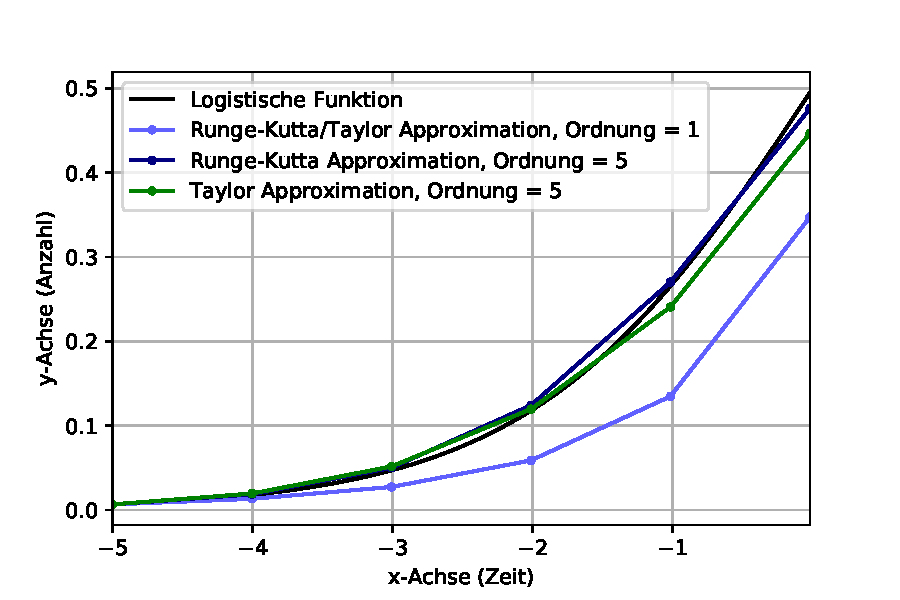
\includegraphics[width=12cm]{papers/taylor/taylorPictures/LogisticFunction.pdf}
	\caption{Gleichung und Approximationen der Logistische Funktion für $k=1$, Approximationen mit 5 Schritten von $-5$ bis $-0.02$ und Startwert der selbe wie bei $k=1$}
	\label{taylor:section:fig:LogisticFunctionApproximation}
	\end{center}
\end{figure}

\begin{table}
\begin{tabular}[h]{@{\hskip1pt}>{$}r<{$}|l|l|l|l|l@{\hskip1pt}}
\hline
n & $m = 1$ & $m = 2$ & $m = 3$ & $m = 4$ & $m = 5$\\
\hline
1 & $0.45519$ & $0.31990$ & $0.11077$ & $4.68470\cdot 10^{-2}$ & $6.19930\cdot 10^{-2}$\\
2 & $0.38755$ & $3.85299\cdot 10^{-2}$ & $5.97521\cdot 10^{-2}$ & $1.05400\cdot 10^{-2}$ & $4.07133\cdot 10^{-2}$\\
5 & $0.14751$ & $2.39004\cdot 10^{-2}$ & $2.59349\cdot 10^{-2}$ & $1.33486\cdot 10^{-2}$ & $1.88327\cdot 10^{-2}$\\
10 & $6.88690\cdot 10^{-2}$ & $4.37589\cdot 10^{-3}$ & $4.37432\cdot 10^{-3}$ & $2.58736\cdot 10^{-3}$ & $3.50711\cdot 10^{-3}$\\
1000 & $6.19312\cdot 10^{-4}$ & $5.23506\cdot 10^{-7}$ & $1.84704\cdot 10^{-7}$ & $1.85763\cdot 10^{-7}$ & $1.85765\cdot 10^{-7}$\\
100000 & $6.18453\cdot 10^{-6}$ & $5.13468\cdot 10^{-11}$ & $1.96497\cdot 10^{-11}$ & $1.96507\cdot 10^{-11}$ & $1.96507\cdot 10^{-11}$\\
\hline
\end{tabular}

\caption{Fehler der numerischen Lösung einer Differentialgleichung nach dem
Runge-Kutta-Verfahren: $m$ = Ordnung, $n$ = Schritte, Start = $-5$, Ende = $-0.02$, (letzte Ziffer abgerundet)
\label{taylor:section:tablerunge}}
\end{table}

\begin{table}
\begin{tabular}[h]{@{\hskip1pt}>{$}r<{$}|l|l|l|l|l@{\hskip1pt}}
\hline
n & $m = 1$ & $m = 2$ & $m = 3$ & $m = 4$ & $m = 5$\\
\hline
1 & $0.45519$ & $0.27840$ & $0.27948$ & $0.29078$ & $0.29515$\\
2 & $0.38755$ & $0.20040$ & $0.19400$ & $0.19579$ & $0.19663$\\
5 & $0.14751$ & $5.30816\cdot 10^{-2}$ & $4.80256\cdot 10^{-2}$ & $4.79241\cdot 10^{-2}$ & $4.79851\cdot 10^{-2}$\\
10 & $6.88690\cdot 10^{-2}$ & $1.60657\cdot 10^{-2}$ & $1.38830\cdot 10^{-2}$ & $1.38673\cdot 10^{-2}$ & $1.38751\cdot 10^{-2}$\\
1000 & $6.19312\cdot 10^{-4}$ & $2.11126\cdot 10^{-6}$ & $1.90164\cdot 10^{-6}$ & $1.90183\cdot 10^{-6}$ & $1.90183\cdot 10^{-6}$\\
100000 & $6.18453\cdot 10^{-6}$ & $2.10965\cdot 10^{-10}$ & $1.90226\cdot 10^{-10}$ & $1.90226\cdot 10^{-10}$ & $1.90226\cdot 10^{-10}$\\
\hline
\end{tabular}

\caption{Fehler der numerischen Lösung einer Differentialgleichung nach dem
Taylor-Verfahren:
$m$ = Ordnung, $n$ = Schritte, Start = $-5$, Ende = $-0.02$, (letzte Ziffer abgerundet)
\label{taylor:section:tabletaylor}}
\end{table}

\begin{figure}
	\centering
	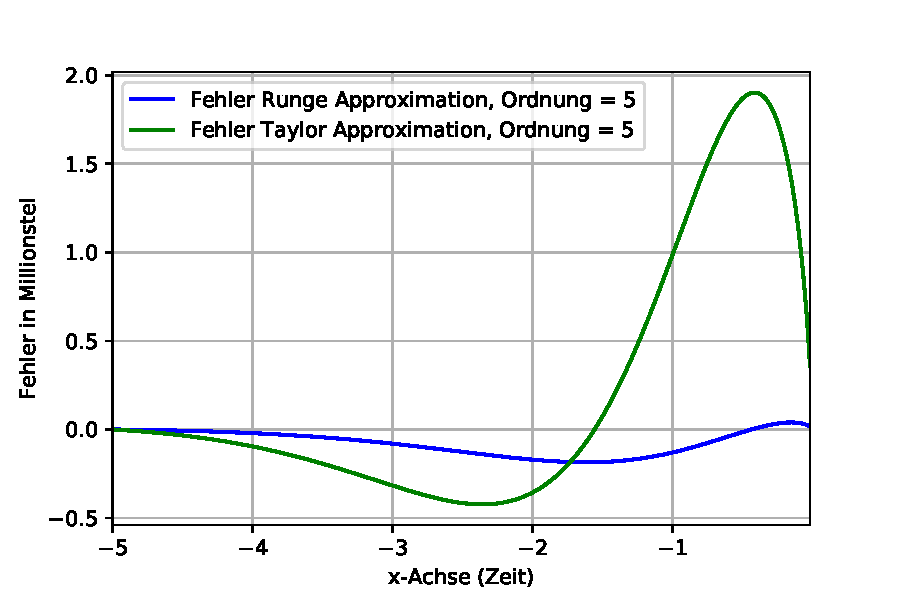
\includegraphics[width=12cm]{papers/taylor/taylorPictures/FehlerRungeUndTaylor.pdf}
	\caption{Fehler der Approximationen bei 1000 Schritten von $-5$ bis $-0.02$ und Startwert der selbe wie bei $m=1$}
	\label{taylor:section:fig:FehlerRungeTaylor}
\end{figure}

\subsection{Auswertung des Vergleiches}
\label{taylor:subsection:Auswertung}
Die ersten Spalten der beiden Tabellen \ref{taylor:section:tablerunge} und \ref{taylor:section:tabletaylor} der beiden Verfahren sehen gleich aus.
Das ist so, weil die Approximationen erster Ordnung auf das selbe herauskommen, nämlich auf das Approximieren der Funktion mit Geraden erster Ordnung.
Das entspricht der Steigung im Auswertungspunkt.

Beim Punkt $n=1$ und $m=2$ ist die Taylor-Approximation besser als Runge-Kutta.
Eine Approximation mit dem Grad 2 und einem Schritt über eine sich so stark verändernde Kurve ist aber eher ein Glückstreffer als ein mathematischer Erfolg.
Es kann gesagt werden, dass das Runge-Kutta-Verfahren in diesem Fall ein kleineren Fehler aufweist. Dies ist auch in der Abbildung \ref{taylor:section:fig:FehlerRungeTaylor} zu sehen.

\section{Probleme mit der logistischen Funktion}
\label{taylor:subsection:Probleme}
Die logistische Funktion wurde gewählt, weil es eine anschauliche, nichtlineare Differentialgleichung ist welche sich somit gut eignet, um das Runge-Kutta-Verfahren mit dem Taylor-Verfahren zu vergleichen.
Dabei traten allerdings folgende zwei Probleme auf.

\subsection{Konvergenz
\label{taylor:subsection:Konvergenz}}
\index{Konvergenz}%
Wie in Abbildung 
\ref{taylor:section:fig:DGLDarstellung}
ersichtlich ist, läuft die Lösung der Differentialgleichung im Punkt 0 gegen 0.5 und bei $\infty$ gegen 1.
Wird nun also diese Differentialgleichung approximiert, dann ist sowieso klar auf welchem Wert wir ungefähr landen werden.
Um eine aussagekräftige Antwort auf die Frage der Qualität der Approximation geben zu können wurden in Abbildung \ref{taylor:section:fig:FehlerRungeTaylor} die Fehler über den ganzen Verlauf der Approximation verglichen.

\subsection{Gefährliche Umgebung der Anfangsbedingung
\label{taylor:subsection:0Punkt}}
Wie in Abbildung 
\ref{taylor:section:fig:DGLDarstellung}
klar dargestellt ist, ist die Ableitung in direkter Umgebung von der gewählten Anfangsbedingung (0, 0.5) zwischen 0 und $\infty$ da der Punkt in der Lösung der Differentialgleichung einer Polstelle entspricht.
Wenn also eine Approximation der Differentialgleichung durch diesen Punkt verläuft, oder auch nur in seine unmittelbare Umgebung kommt kann die Approximation komplett anders weiter verlaufen als man erwarten würde.
Dies liegt daran, dass selbst kleine Fehler, welche eine Approximation zwangsweise haben muss, sich in der Nähe des Punktes sehr stark auf den weiteren Verlauf auswirken.
Um dies zu umgehen wurde die nähere Umgebung dieses Wendepunkts einfach aus der Approximation ausgeschlossen indem nur bis 0.02 davor approximiert wurde.
Man könnte nun aber die erhaltenen linke Kurve an dem Wendepunkt punktspiegeln und hätte so die zweite Hälfte ebenfalls, welche durch die Spiegelung sowieso redundant und für uns deshalb nicht interessant wäre.

%\nameref
%\pageref{}
%\numref
%\ref{taylor:section:loesung}.
%\ref{taylor:section:folgerung}.


